% ============================================================================
% CHƯƠNG I: TỔNG QUAN VỀ HỆ THỐNG
% ============================================================================
\chapter{TỔNG QUAN VỀ HỆ THỐNG}

\section{Giới thiệu bài toán và mục tiêu hệ thống}

\subsection{Bối cảnh và đặt vấn đề}

Trong bối cảnh số hóa và phát triển công nghệ thông tin, các thư viện truyền thống đang dần chuyển đổi sang mô hình thư viện điện tử (e-Library). Đối với các hệ thống thư viện có nhiều chi nhánh phân bố ở các vị trí địa lý khác nhau, việc quản lý tập trung và đồng bộ dữ liệu trở thành một thách thức lớn.

Các vấn đề cần giải quyết:
\begin{itemize}
    \item \textbf{Tính phân tán}: Dữ liệu cần được lưu trữ và truy cập từ nhiều vị trí địa lý khác nhau
    \item \textbf{Tính sẵn sàng cao}: Hệ thống phải hoạt động liên tục, có khả năng tự phục hồi khi gặp sự cố
    \item \textbf{Hiệu năng}: Đảm bảo thời gian phản hồi nhanh cho các truy vấn dữ liệu
    \item \textbf{Khả năng mở rộng}: Hệ thống có thể scale theo chiều ngang khi lượng dữ liệu tăng
\end{itemize}

\subsection{Mục tiêu của đề tài}

Đề tài \textbf{"Xây dựng hệ thống E-Library Phân tán nhiều cơ sở"} hướng đến các mục tiêu sau:

\begin{enumerate}
    \item \textbf{Thiết kế và cài đặt hệ thống phân tán}:
    \begin{itemize}
        \item Kiến trúc 4 node: 1 Central Hub + 3 chi nhánh (Hà Nội, Đà Nẵng, TP.HCM)
        \item Sử dụng MongoDB Replica Set cho high availability
        \item Hỗ trợ Zone Sharding theo vùng địa lý
    \end{itemize}

    \item \textbf{Triển khai các kỹ thuật NoSQL nâng cao}:
    \begin{itemize}
        \item Aggregation Pipeline với 10+ operators
        \item Map-Reduce cho phân tích dữ liệu phức tạp
        \item Full-text Search với TEXT index
    \end{itemize}

    \item \textbf{Đảm bảo bảo mật và phân quyền}:
    \begin{itemize}
        \item JWT (JSON Web Token) authentication
        \item Role-based Access Control (RBAC)
        \item Password hashing với bcrypt
    \end{itemize}

    \item \textbf{Xây dựng giao diện quản trị}:
    \begin{itemize}
        \item Dashboard thống kê với Chart.js
        \item CRUD đầy đủ cho sách, người dùng, đơn hàng
        \item Responsive design với Bootstrap 5
    \end{itemize}
\end{enumerate}

\section{Tổng quan về hệ thống e-Library}

\subsection{Mô hình hệ thống phân tán}

Hệ thống e-Library được thiết kế theo mô hình phân tán với 4 node độc lập, mỗi node có database riêng nhưng được đồng bộ qua MongoDB Replica Set:

\begin{table}[H]
\centering
\caption{Các node trong hệ thống e-Library}
\label{tab:nodes}
\begin{tabular}{|c|l|l|c|l|}
\hline
\textbf{STT} & \textbf{Node} & \textbf{Database} & \textbf{Port} & \textbf{Vai trò} \\
\hline
1 & Central Hub & Nhasach & 8001 & Trung tâm quản lý \\
2 & Branch Hà Nội & NhasachHaNoi & 8002 & Chi nhánh miền Bắc \\
3 & Branch Đà Nẵng & NhasachDaNang & 8003 & Chi nhánh miền Trung \\
4 & Branch TP.HCM & NhasachHoChiMinh & 8004 & Chi nhánh miền Nam \\
\hline
\end{tabular}
\end{table}

\subsection{Dữ liệu thực tế trong hệ thống}

Tính đến thời điểm hoàn thành đề tài, hệ thống có các số liệu sau:

\begin{table}[H]
\centering
\caption{Thống kê dữ liệu theo từng chi nhánh}
\label{tab:data_stats}
\begin{tabular}{|l|r|r|r|}
\hline
\textbf{Chi nhánh} & \textbf{Số sách} & \textbf{Số users} & \textbf{Số orders} \\
\hline
Central Hub (Nhasach) & 509 & 42 & 111 \\
Chi nhánh Hà Nội & 200 & 13 & 46 \\
Chi nhánh Đà Nẵng & 163 & 12 & 16 \\
Chi nhánh TP.HCM & 146 & 11 & 14 \\
\hline
\textbf{Tổng cộng} & \textbf{1.018} & \textbf{78} & \textbf{187} \\
\hline
\end{tabular}
\end{table}

\subsection{Kiến trúc tổng quan}

\begin{figure}[H]
\centering
\begin{tikzpicture}[
    node distance=1.5cm,
    box/.style={rectangle, draw, rounded corners, minimum width=3.2cm, minimum height=1.1cm, align=center, font=\small},
    db/.style={cylinder, draw, shape border rotate=90, minimum width=2cm, minimum height=1.2cm, aspect=0.25, font=\scriptsize, align=center},
    arrow/.style={->, >=stealth, thick}
]
    % Client Layer
    \node[box, fill=blue!15, drop shadow] (client) at (0,6) {\textbf{Web Browser}\\Admin/Customer};

    % PHP Application Layer - Central Hub
    \node[box, fill=green!25, drop shadow] (central) at (0,4) {\textbf{Central Hub}\\PHP 8.4 | Port 8001\\DB: Nhasach};

    % PHP Application Layer - Branches
    \node[box, fill=green!15] (hanoi) at (-5,2) {\textbf{Chi nhánh HN}\\Port 8002\\DB: NhasachHaNoi};
    \node[box, fill=green!15] (danang) at (0,2) {\textbf{Chi nhánh ĐN}\\Port 8003\\DB: NhasachDaNang};
    \node[box, fill=green!15] (hcm) at (5,2) {\textbf{Chi nhánh HCM}\\Port 8004\\DB: NhasachHoChiMinh};

    % MongoDB Layer - 4 separate databases
    \node[db, fill=orange!20] (mongo1) at (-5,0) {MongoDB\\mongo1\\:27017\\Nhasach};
    \node[db, fill=orange!15] (mongo2) at (-1.5,0) {MongoDB\\mongo2\\:27018\\NhasachHaNoi};
    \node[db, fill=orange!15] (mongo3) at (1.5,0) {MongoDB\\mongo3\\:27019\\NhasachDaNang};
    \node[db, fill=orange!15] (mongo4) at (5,0) {MongoDB\\mongo4\\:27020\\NhasachHoChiMinh};

    % Connections - Client to Central
    \draw[arrow, blue, line width=1.2pt] (client) -- (central);

    % Connections - Central to Branches (sync)
    \draw[arrow, red, dashed, line width=1pt] (central) -- node[left, font=\tiny] {sync} (hanoi);
    \draw[arrow, red, dashed, line width=1pt] (central) -- node[right, font=\tiny] {sync} (danang);
    \draw[arrow, red, dashed, line width=1pt] (central) -- node[right, font=\tiny] {sync} (hcm);

    % Connections - PHP to MongoDB
    \draw[arrow, green!60!black, line width=1pt] (central) -- (mongo1);
    \draw[arrow, green!60!black, line width=1pt] (hanoi) -- (mongo2);
    \draw[arrow, green!60!black, line width=1pt] (danang) -- (mongo3);
    \draw[arrow, green!60!black, line width=1pt] (hcm) -- (mongo4);

    % Labels
    \node[font=\tiny, text=gray] at (0,-1.2) {Mỗi chi nhánh có database MongoDB riêng biệt};

\end{tikzpicture}
\caption{Kiến trúc tổng quan hệ thống e-Library phân tán 4 cơ sở}
\label{fig:architecture}
\end{figure}

\section{Một số khái niệm và nghiệp vụ liên quan}

\subsection{Khái niệm về các đối tượng}

\begin{enumerate}
    \item \textbf{Quản trị viên hệ thống (Admin)}:
    \begin{itemize}
        \item Toàn quyền quản lý hệ thống tại Central Hub
        \item Quản lý sách, người dùng, đơn hàng
        \item Xem Dashboard thống kê
        \item Đồng bộ dữ liệu giữa các chi nhánh
    \end{itemize}

    \item \textbf{Quản trị viên chi nhánh (Branch Admin)}:
    \begin{itemize}
        \item Quản lý sách tại chi nhánh được phân công
        \item Username: adminHN, adminDN, adminHCM
        \item Không thể can thiệp vào chi nhánh khác
    \end{itemize}

    \item \textbf{Khách hàng (Customer)}:
    \begin{itemize}
        \item Đăng ký tài khoản tại chi nhánh
        \item Tìm kiếm, xem thông tin sách
        \item Mượn sách qua giỏ hàng
        \item Xem lịch sử mượn sách
    \end{itemize}
\end{enumerate}

\subsection{Các quy trình nghiệp vụ}

\begin{enumerate}
    \item \textbf{Quy trình đăng ký/đăng nhập}:
    \begin{itemize}
        \item Khách hàng đăng ký với username, password, email
        \item Mật khẩu được hash bằng bcrypt (cost factor 12)
        \item Đăng nhập tạo JWT token với thời hạn 24 giờ
        \item Token được lưu trong session hoặc Authorization header
    \end{itemize}

    \item \textbf{Quy trình tìm kiếm sách}:
    \begin{itemize}
        \item Hỗ trợ Full-text Search với TEXT index
        \item Tìm theo tên sách, thể loại, tác giả
        \item Kết quả được sắp xếp theo relevance score
        \item Hỗ trợ phân trang với 20 sách/trang
    \end{itemize}

    \item \textbf{Quy trình mượn sách}:
    \begin{itemize}
        \item Khách hàng thêm sách vào giỏ hàng
        \item Chọn số ngày mượn, hệ thống tính tiền
        \item Xác nhận đơn mượn, trừ số dư
        \item Trạng thái đơn: pending $\rightarrow$ paid $\rightarrow$ success $\rightarrow$ returned
    \end{itemize}

    \item \textbf{Quy trình đồng bộ dữ liệu}:
    \begin{itemize}
        \item Chi nhánh gửi dữ liệu về Central Hub qua REST API
        \item Sử dụng script \texttt{sync\_data.sh} để đồng bộ
        \item Dữ liệu customers và orders được tổng hợp tại Central
    \end{itemize}
\end{enumerate}

\section{Một số công nghệ được áp dụng}

\subsection{PHP 8.4 và MongoDB Driver}

PHP (Hypertext Preprocessor) là ngôn ngữ lập trình kịch bản phía server, được sử dụng rộng rãi trong phát triển ứng dụng web. Trong đề tài này, nhóm sử dụng \textbf{PHP 8.4} kết hợp với thư viện \texttt{mongodb/mongodb v2.1}.

\textbf{Đặc điểm của mongodb/mongodb library}:
\begin{itemize}
    \item Hỗ trợ đầy đủ CRUD operations với type-safe API
    \item Aggregation Pipeline Builder cho truy vấn phức tạp
    \item Hỗ trợ BSON types (ObjectId, UTCDateTime, Javascript)
    \item Connection pooling tự động
    \item Read/Write Concern configuration
\end{itemize}

\textbf{Cấu hình kết nối trong Connection.php}:

File \texttt{Connection.php} là điểm trung tâm quản lý kết nối đến MongoDB cho toàn bộ ứng dụng. File này hỗ trợ 3 chế độ kết nối: \textbf{standalone} (một máy chủ đơn), \textbf{replicaset} (cluster 3 nodes với failover tự động), và \textbf{sharded} (phân mảnh dữ liệu theo vùng). Tham số \texttt{readPreference: primaryPreferred} cho phép đọc từ Secondary nếu Primary quá tải, còn \texttt{w: majority} đảm bảo dữ liệu được ghi vào đa số nodes trước khi xác nhận thành công - đây là chiến lược cân bằng giữa hiệu năng và độ tin cậy.

\begin{lstlisting}[language=PHP, caption=Connection.php - Cấu hình kết nối MongoDB]
<?php
require 'vendor/autoload.php';
use MongoDB\Client;

$MODE = 'sharded'; // Options: standalone, replicaset, sharded
$Database = "Nhasach";

switch ($MODE) {
    case 'sharded':
        $conn = new Client("mongodb://localhost:27017", [
            'readPreference' => 'primaryPreferred',
            'w' => 'majority',
            'journal' => true
        ]);
        break;
    case 'replicaset':
        $conn = new Client(
            "mongodb://mongo1:27017,mongo2:27017,mongo3:27017/?replicaSet=rs0",
            ['readPreference' => 'primaryPreferred', 'w' => 'majority']
        );
        break;
    default:
        $conn = new Client("mongodb://localhost:27017");
}
$db = $conn->$Database;
\end{lstlisting}

\subsection{MongoDB và MongoDB Compass}

\textbf{MongoDB} là hệ quản trị cơ sở dữ liệu NoSQL hướng tài liệu (document-oriented), lưu trữ dữ liệu dưới dạng BSON (Binary JSON). Phiên bản sử dụng: \textbf{MongoDB 4.4} (Docker image).

\textbf{Các tính năng MongoDB được sử dụng trong đề tài}:
\begin{itemize}
    \item \textbf{Replica Set}: 3 nodes (mongo1, mongo2, mongo3) với automatic failover
    \item \textbf{Aggregation Pipeline}: 10+ operators (\$match, \$group, \$sort, \$lookup, \$facet, \$bucket...)
    \item \textbf{Map-Reduce}: 5 operations cho phân tích phức tạp
    \item \textbf{TEXT Index}: Full-text search tiếng Việt
    \item \textbf{Compound Index}: Tối ưu shard-aware queries
\end{itemize}

\textbf{MongoDB Compass} là công cụ GUI chính thức, hỗ trợ:
\begin{itemize}
    \item Trực quan hóa dữ liệu và cấu trúc schema
    \item Aggregation Pipeline Builder với drag-and-drop
    \item Explain Plan để phân tích query performance
    \item Real-time server statistics
\end{itemize}

\subsection{Docker và Docker Compose}

\textbf{Docker} là nền tảng container hóa cho phép đóng gói ứng dụng cùng dependencies. \textbf{Docker Compose} cho phép định nghĩa multi-container applications.

\textbf{Vai trò trong đề tài}:
\begin{itemize}
    \item Khởi tạo MongoDB Replica Set với 3 containers
    \item Mạng nội bộ \texttt{mongo-net} cho giao tiếp giữa các nodes
    \item Volume persistence cho dữ liệu (\texttt{mongo1\_data}, \texttt{mongo2\_data}, \texttt{mongo3\_data})
    \item Dễ dàng tái lập kịch bản Failover testing
\end{itemize}

Đoạn cấu hình Docker Compose dưới đây định nghĩa một MongoDB Replica Set gồm 3 containers: \texttt{mongo1} (Primary, cổng 27017), \texttt{mongo2} và \texttt{mongo3} (Secondary, cổng 27018 và 27019). Tham số \texttt{--replSet rs0} cho biết cả 3 containers thuộc cùng một replica set tên ``rs0''. Mạng \texttt{mongo-net} với driver \texttt{bridge} cho phép các containers giao tiếp nội bộ. Khi \texttt{mongo1} gặp sự cố, một trong hai Secondary sẽ tự động được bầu làm Primary mới trong vòng 10-12 giây.

\begin{lstlisting}[caption=docker-compose.yml - MongoDB Replica Set]
version: '3.8'
services:
  mongo1:
    image: mongo:4.4
    container_name: mongo1
    ports: ["27017:27017"]
    command: ["mongod", "--replSet", "rs0", "--bind_ip_all"]
    volumes: [mongo1_data:/data/db]
    networks: [mongo-net]

  mongo2:
    image: mongo:4.4
    ports: ["27018:27017"]
    command: ["mongod", "--replSet", "rs0", "--bind_ip_all"]
    depends_on: [mongo1]

  mongo3:
    image: mongo:4.4
    ports: ["27019:27017"]
    command: ["mongod", "--replSet", "rs0", "--bind_ip_all"]
    depends_on: [mongo1]

networks:
  mongo-net:
    driver: bridge
\end{lstlisting}

\subsection{JWT (JSON Web Token)}

JWT là chuẩn mở (RFC 7519) để truyền thông tin an toàn giữa các bên dưới dạng JSON object. Thư viện \texttt{firebase/php-jwt v6.x} được sử dụng.

\textbf{Cấu trúc JWT trong hệ thống}:
\begin{itemize}
    \item \textbf{Header}: Algorithm HS256
    \item \textbf{Payload}: user\_id, username, role, node\_id, iat, exp
    \item \textbf{Signature}: HMAC-SHA256 với secret key
\end{itemize}

\begin{lstlisting}[language=PHP, caption=JWTHelper.php - Tạo JWT Token]
public static function generateToken($userId, $username, $role, $nodeId = null) {
    $payload = [
        'iss' => JWT_ISSUER,
        'iat' => time(),
        'exp' => time() + (24 * 3600), // 24 hours
        'nbf' => time(),
        'data' => [
            'user_id'  => $userId,
            'username' => $username,
            'role'     => $role,
            'node_id'  => $nodeId ?? JWT_NODE_ID
        ]
    ];
    return JWT::encode($payload, JWT_SECRET_KEY, 'HS256');
}
\end{lstlisting}

\subsection{Chart.js}

Chart.js là thư viện JavaScript mã nguồn mở để vẽ biểu đồ. Phiên bản 4.4 được sử dụng cho Dashboard.

\textbf{Các loại biểu đồ được sử dụng}:
\begin{itemize}
    \item \textbf{Bar Chart}: Số lượng sách theo chi nhánh, top sách được mượn
    \item \textbf{Pie/Doughnut Chart}: Phân bố người dùng theo role, trạng thái đơn hàng
    \item \textbf{Line Chart}: Xu hướng mượn sách theo thời gian
\end{itemize}

% ============================================================================
% CHƯƠNG II: PHÂN TÍCH VÀ THIẾT KẾ HỆ THỐNG
% ============================================================================
\chapter{PHÂN TÍCH VÀ THIẾT KẾ HỆ THỐNG}

\section{Xác định các yêu cầu}

\subsection{Yêu cầu phi chức năng}

\begin{enumerate}
    \item \textbf{Tính sẵn sàng cao (High Availability)}:
    \begin{itemize}
        \item Hệ thống hoạt động 24/7
        \item Tự động failover khi 1/3 nodes gặp sự cố
        \item Recovery time: 10-15 giây
    \end{itemize}

    \item \textbf{Hiệu năng (Performance)}:
    \begin{itemize}
        \item Thời gian phản hồi trung bình < 3ms
        \item Throughput: 500+ ops/sec
        \item Hỗ trợ concurrent users
    \end{itemize}

    \item \textbf{Khả năng mở rộng (Scalability)}:
    \begin{itemize}
        \item Horizontal scaling: thêm shard không cần downtime
        \item Zone-based sharding theo địa lý
    \end{itemize}

    \item \textbf{Bảo mật (Security)}:
    \begin{itemize}
        \item JWT authentication với expiration
        \item bcrypt password hashing (cost 12)
        \item RBAC: admin/customer roles
        \item Brute-force protection
    \end{itemize}

    \item \textbf{Nhất quán dữ liệu (Consistency)}:
    \begin{itemize}
        \item Write Concern: majority
        \item Read Preference: primaryPreferred
        \item Replication lag < 500ms
    \end{itemize}
\end{enumerate}

\subsection{Yêu cầu chức năng}

\begin{table}[H]
\centering
\caption{Danh sách yêu cầu chức năng}
\label{tab:functional_req}
\begin{tabular}{|c|l|l|l|}
\hline
\textbf{STT} & \textbf{Chức năng} & \textbf{Actor} & \textbf{Mô tả} \\
\hline
1 & Đăng ký tài khoản & Customer & Tạo account mới \\
2 & Đăng nhập/Đăng xuất & All & JWT authentication \\
3 & Quản lý sách (CRUD) & Admin & Thêm/Sửa/Xóa sách \\
4 & Tìm kiếm sách & All & Full-text search \\
5 & Quản lý người dùng & Admin & CRUD users \\
6 & Giỏ hàng & Customer & Thêm/Xóa sách \\
7 & Đặt mượn sách & Customer & Tạo đơn mượn \\
8 & Lịch sử mượn & Customer & Xem orders \\
9 & Dashboard thống kê & Admin & Charts, reports \\
10 & Đồng bộ dữ liệu & System & Sync branches \\
\hline
\end{tabular}
\end{table}

\section{Ca sử dụng - Use Case}

\subsection{Danh sách các tác nhân}

\begin{table}[H]
\centering
\caption{Danh sách tác nhân trong hệ thống}
\begin{tabular}{|c|l|l|}
\hline
\textbf{STT} & \textbf{Tác nhân} & \textbf{Mô tả} \\
\hline
1 & Admin & Quản trị viên, toàn quyền hệ thống \\
2 & Customer & Khách hàng, mượn/trả sách \\
3 & System & Hệ thống tự động (sync, cron jobs) \\
\hline
\end{tabular}
\end{table}

\subsection{Biểu đồ Use Case tổng quát}

\begin{figure}[H]
\centering
\begin{tikzpicture}[
    actor/.style={circle, draw, minimum size=0.6cm, font=\tiny},
    usecase/.style={ellipse, draw, minimum width=2cm, minimum height=0.8cm, align=center, font=\scriptsize},
    node distance=0.8cm
]
    % Actors
    \node[actor] (admin) at (-6,0) {};
    \node[below=0.05cm of admin, font=\scriptsize] {Admin};

    \node[actor] (customer) at (-6,-5) {};
    \node[below=0.05cm of customer, font=\scriptsize] {Customer};

    % System boundary
    \draw[dashed, rounded corners] (-3.5,-7) rectangle (4,1.5);
    \node[font=\small] at (0.25,1) {\textbf{e-Library System}};

    % Use cases - Admin
    \node[usecase, fill=blue!10] (login) at (0,0.3) {Đăng nhập};
    \node[usecase, fill=blue!10] (dashboard) at (0,-0.8) {Dashboard};
    \node[usecase, fill=blue!10] (manage_books) at (0,-1.9) {Quản lý sách};
    \node[usecase, fill=blue!10] (manage_users) at (0,-3) {Quản lý users};

    % Use cases - Customer
    \node[usecase, fill=green!10] (search) at (2.5,-1.9) {Tìm kiếm sách};
    \node[usecase, fill=green!10] (cart) at (2.5,-3) {Giỏ hàng};
    \node[usecase, fill=green!10] (order) at (0,-4.2) {Đặt mượn};
    \node[usecase, fill=green!10] (history) at (0,-5.4) {Lịch sử};
    \node[usecase, fill=green!10] (browse) at (2.5,-4.2) {Xem sách};

    % Connections - Admin
    \draw (admin) -- (login);
    \draw (admin) -- (dashboard);
    \draw (admin) -- (manage_books);
    \draw (admin) -- (manage_users);

    % Connections - Customer
    \draw (customer) -- (login);
    \draw (customer) -- (search);
    \draw (customer) -- (cart);
    \draw (customer) -- (order);
    \draw (customer) -- (history);
    \draw (customer) -- (browse);

\end{tikzpicture}
\caption{Biểu đồ Use Case tổng quát}
\label{fig:usecase}
\end{figure}

\section{Mô hình cấu trúc}

\subsection{Danh sách các lớp đối tượng}

Từ phân tích yêu cầu, hệ thống bao gồm 5 lớp đối tượng chính:

\begin{enumerate}
    \item \textbf{User}: Quản lý thông tin người dùng
    \begin{itemize}
        \item Thuộc tính: \_id, username, password, fullname, email, role, balance, location, status, created\_at
        \item Phương thức: register(), login(), logout(), updateProfile(), changePassword()
    \end{itemize}

    \item \textbf{Book}: Quản lý thông tin sách
    \begin{itemize}
        \item Thuộc tính: \_id, bookCode, bookName, bookGroup, author, description, quantity, pricePerDay, borrowCount, location, status
        \item Phương thức: create(), update(), delete(), search(), getByLocation()
    \end{itemize}

    \item \textbf{Cart}: Quản lý giỏ hàng
    \begin{itemize}
        \item Thuộc tính: \_id, user\_id, items[], total\_quantity, total\_amount, updated\_at
        \item Phương thức: addItem(), removeItem(), updateQuantity(), clear(), checkout()
    \end{itemize}

    \item \textbf{Order}: Quản lý đơn mượn sách
    \begin{itemize}
        \item Thuộc tính: \_id, user\_id, username, items[], total\_quantity, total\_amount, status, borrow\_date, return\_date, created\_at
        \item Phương thức: create(), updateStatus(), calculateFee(), getByUser()
    \end{itemize}

    \item \textbf{Activity}: Ghi log hoạt động
    \begin{itemize}
        \item Thuộc tính: \_id, action, user\_id, details, ip\_address, timestamp
        \item Phương thức: log(), getByUser(), getByAction(), getRecent()
    \end{itemize}
\end{enumerate}

\subsection{Biểu đồ lớp}

\begin{figure}[H]
\centering
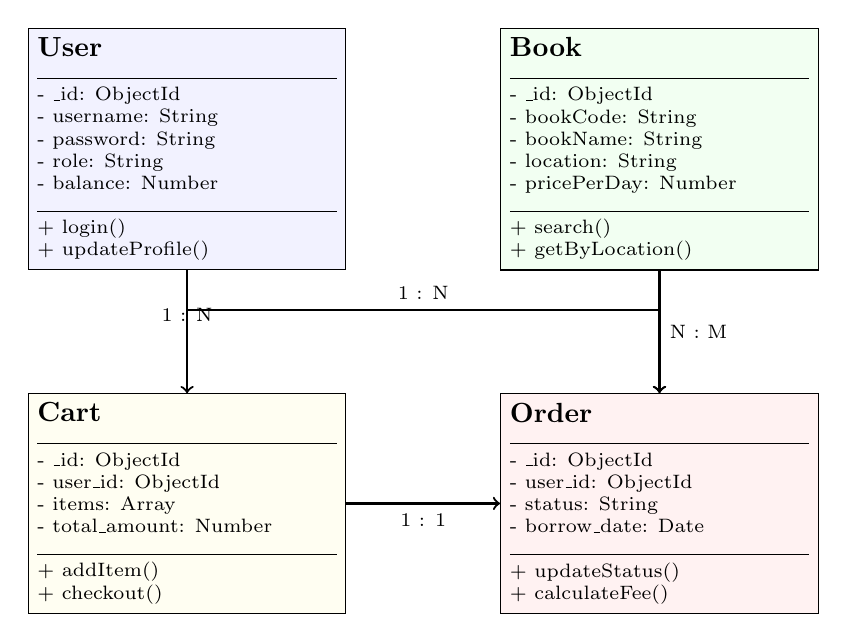
\begin{tikzpicture}[
    class/.style={rectangle, draw, minimum width=4cm, minimum height=2.5cm, align=left, font=\scriptsize},
    node distance=1cm
]
    % Classes
    \node[class, fill=blue!5] (user) at (0,0) {
        \textbf{\normalsize User}\\
        \rule{3.8cm}{0.3pt}\\
        - \_id: ObjectId\\
        - username: String\\
        - password: String\\
        - role: String\\
        - balance: Number\\
        \rule{3.8cm}{0.3pt}\\
        + login()\\
        + updateProfile()
    };

    \node[class, fill=green!5] (book) at (6,0) {
        \textbf{\normalsize Book}\\
        \rule{3.8cm}{0.3pt}\\
        - \_id: ObjectId\\
        - bookCode: String\\
        - bookName: String\\
        - location: String\\
        - pricePerDay: Number\\
        \rule{3.8cm}{0.3pt}\\
        + search()\\
        + getByLocation()
    };

    \node[class, fill=yellow!5] (cart) at (0,-4.5) {
        \textbf{\normalsize Cart}\\
        \rule{3.8cm}{0.3pt}\\
        - \_id: ObjectId\\
        - user\_id: ObjectId\\
        - items: Array\\
        - total\_amount: Number\\
        \rule{3.8cm}{0.3pt}\\
        + addItem()\\
        + checkout()
    };

    \node[class, fill=red!5] (order) at (6,-4.5) {
        \textbf{\normalsize Order}\\
        \rule{3.8cm}{0.3pt}\\
        - \_id: ObjectId\\
        - user\_id: ObjectId\\
        - status: String\\
        - borrow\_date: Date\\
        \rule{3.8cm}{0.3pt}\\
        + updateStatus()\\
        + calculateFee()
    };

    % Relationships
    \draw[->, thick] (user) -- node[above, font=\scriptsize] {1 : N} (cart);
    \draw[->, thick] (user.south) -- ++(0,-0.5) -| node[near start, above, font=\scriptsize] {1 : N} (order.north);
    \draw[->, thick] (book) -- node[right, font=\scriptsize] {N : M} (order);
    \draw[->, thick] (cart) -- node[below, font=\scriptsize] {1 : 1} (order);

\end{tikzpicture}
\caption{Biểu đồ lớp hệ thống e-Library}
\label{fig:class_diagram}
\end{figure}

\section{Thiết kế CSDL}

\subsection{Xác định các collection}

\begin{table}[H]
\centering
\caption{Danh sách collection trong MongoDB}
\begin{tabular}{|c|l|l|l|}
\hline
\textbf{STT} & \textbf{Collection} & \textbf{Mô tả} & \textbf{Documents} \\
\hline
1 & users & Thông tin người dùng & 78 \\
2 & books & Danh mục sách & 1.018 \\
3 & carts & Giỏ hàng & Dynamic \\
4 & orders & Đơn mượn sách & 187 \\
5 & activities & Log hoạt động & Dynamic \\
6 & customers & Tổng hợp KH (Central) & 78 \\
\hline
\end{tabular}
\end{table}

\subsection{Mối quan hệ giữa các collection}

Trong MongoDB, các collection không có ràng buộc khóa ngoại như trong cơ sở dữ liệu quan hệ. Tuy nhiên, các mối quan hệ logic vẫn được duy trì thông qua việc lưu trữ tham chiếu (reference) hoặc nhúng dữ liệu (embedded documents). Bảng \ref{tab:collection_relations} mô tả các mối quan hệ giữa các collection trong hệ thống:

\begin{table}[H]
\centering
\caption{Mối quan hệ giữa các collection}
\label{tab:collection_relations}
\begin{tabular}{|l|c|p{7cm}|}
\hline
\textbf{Collection} & \textbf{Quan hệ} & \textbf{Ý nghĩa} \\
\hline
users -- carts & 1:1 & Một người dùng chỉ có một giỏ hàng. Giỏ hàng được tạo tự động khi người dùng thêm sách đầu tiên. \\
\hline
users -- orders & 1:N & Một người dùng có thể tạo nhiều đơn mượn sách. Mỗi đơn mượn lưu user\_id để truy vấn ngược. \\
\hline
carts -- books & N:M & Một giỏ hàng có thể chứa nhiều sách, và một đầu sách có thể xuất hiện trong giỏ hàng của nhiều người dùng cùng lúc (embedded trong items[]). \\
\hline
orders -- books & N:M & Một đơn mượn có thể chứa nhiều sách, và một đầu sách có thể xuất hiện trong nhiều đơn mượn khác nhau (embedded trong items[]). \\
\hline
\end{tabular}
\end{table}

\textbf{Chiến lược thiết kế:} Trong NoSQL, việc thiết kế mối quan hệ khác biệt cơ bản so với SQL truyền thống. Thay vì dùng JOIN, MongoDB cho phép hai cách tiếp cận: \textit{nhúng dữ liệu trực tiếp} (denormalization) hoặc \textit{tham chiếu qua ObjectId} (normalization). Hệ thống e-Library sử dụng kết hợp cả hai để tối ưu hiệu năng:

\begin{itemize}
    \item \textbf{Tham chiếu (Reference):} \texttt{user\_id} trong carts và orders để liên kết với collection users. Khi thông tin user thay đổi (email, số dư), chỉ cần cập nhật một document trong users mà không ảnh hưởng đến các đơn hàng cũ.
    \item \textbf{Nhúng (Embedding):} \texttt{items[]} trong carts và orders chứa snapshot thông tin sách tại thời điểm mượn (tên, giá). Đây là chiến lược ``snapshot data'' - đảm bảo đơn hàng lưu chính xác giá thuê tại thời điểm giao dịch, ngay cả khi giá sách thay đổi sau đó.
\end{itemize}

\subsection{Thiết kế bảng dữ liệu vật lý}

Dưới đây là cấu trúc JSON của các collection chính. Mỗi document trong MongoDB tương đương một bản ghi (row) trong SQL, nhưng linh hoạt hơn vì các trường có thể khác nhau giữa các documents.

\textbf{Collection users:} Lưu thông tin tài khoản với trường \texttt{balance} là số dư ví (đơn vị VND) để thanh toán tiền mượn sách.

\begin{lstlisting}[language=json, caption=Schema collection users]
{
    "_id": ObjectId("..."),
    "username": "admin",           // Unique
    "password": "$2y$12$...",      // bcrypt hash
    "fullname": "Administrator",
    "email": "admin@elibrary.vn",
    "role": "admin",               // admin | customer
    "balance": 500000,
    "location": "Nhasach",
    "status": "active",
    "created_at": ISODate("2026-01-01T00:00:00Z")
}
\end{lstlisting}

\textbf{Collection books:} Trường \texttt{location} là shard key để phân mảnh dữ liệu theo vùng địa lý. Trường \texttt{borrowCount} được tăng mỗi khi có người mượn, dùng để thống kê sách phổ biến.

\begin{lstlisting}[language=json, caption=Schema collection books]
{
    "_id": ObjectId("..."),
    "bookCode": "00001",           // Unique globally
    "bookName": "Lap trinh Python",
    "bookGroup": "Cong nghe",
    "author": "Nguyen Van A",
    "description": "Sach day lap trinh Python...",
    "quantity": 10,
    "pricePerDay": 5000,
    "borrowCount": 25,
    "location": "Ha Noi",          // Shard key
    "status": "active"
}
\end{lstlisting}

\textbf{Collection orders:} Mảng \texttt{items[]} chứa chi tiết sách mượn (nhúng để snapshot dữ liệu). Trạng thái \texttt{status} theo quy trình: pending → paid → success → returned.

\begin{lstlisting}[language=json, caption=Schema collection orders]
{
    "_id": ObjectId("..."),
    "user_id": ObjectId("..."),
    "username": "annv",
    "items": [
        {
            "bookCode": "00001",
            "bookName": "Lap trinh Python",
            "quantity": 1,
            "pricePerDay": 5000,
            "days": 7,
            "subtotal": 35000
        }
    ],
    "total_quantity": 1,
    "total_amount": 35000,
    "status": "success",           // pending|paid|success|returned
    "borrow_date": ISODate("2026-01-01"),
    "return_date": ISODate("2026-01-08"),
    "created_at": ISODate("2026-01-01T10:30:00Z")
}
\end{lstlisting}

\subsection{Thiết kế mô hình phân tán}

Hệ thống e-Library sử dụng kiến trúc phân tán với 4 MongoDB instances độc lập, mỗi instance phục vụ một chi nhánh riêng biệt. Mô hình này đảm bảo:

\begin{itemize}
    \item \textbf{Tính độc lập}: Mỗi chi nhánh có database riêng, không phụ thuộc vào các chi nhánh khác
    \item \textbf{Hiệu năng cao}: Truy vấn trực tiếp vào database local, giảm latency
    \item \textbf{Khả năng mở rộng}: Dễ dàng thêm chi nhánh mới bằng cách deploy MongoDB instance mới
    \item \textbf{Đồng bộ dữ liệu}: Central Hub tổng hợp dữ liệu từ các chi nhánh qua REST API
\end{itemize}

\begin{figure}[H]
\centering
\begin{tikzpicture}[
    container/.style={rectangle, draw, rounded corners, minimum width=2.8cm, minimum height=1.2cm, align=center, font=\small},
    db/.style={cylinder, draw, shape border rotate=90, minimum width=2.2cm, minimum height=1cm, aspect=0.25, font=\scriptsize, align=center},
    node distance=1.2cm
]
    % PHP Applications Layer
    \node[container, fill=green!25, drop shadow] (central) at (0,4) {\textbf{Central Hub}\\Port 8001};
    \node[container, fill=green!15] (hanoi) at (-5,2) {\textbf{Chi nhánh HN}\\Port 8002};
    \node[container, fill=green!15] (danang) at (0,2) {\textbf{Chi nhánh ĐN}\\Port 8003};
    \node[container, fill=green!15] (hcm) at (5,2) {\textbf{Chi nhánh HCM}\\Port 8004};

    % MongoDB Instances
    \node[db, fill=orange!20] (mongo1) at (-5,0) {mongo1\\:27017\\Nhasach};
    \node[db, fill=orange!15] (mongo2) at (-1.5,0) {mongo2\\:27018\\NhasachHaNoi};
    \node[db, fill=orange!15] (mongo3) at (1.5,0) {mongo3\\:27019\\NhasachDaNang};
    \node[db, fill=orange!15] (mongo4) at (5,0) {mongo4\\:27020\\NhasachHoChiMinh};

    % Connections - PHP to MongoDB
    \draw[->, thick, green!60!black] (central) -- (mongo1);
    \draw[->, thick, green!60!black] (hanoi) -- (mongo2);
    \draw[->, thick, green!60!black] (danang) -- (mongo3);
    \draw[->, thick, green!60!black] (hcm) -- (mongo4);

    % Sync connections
    \draw[->, dashed, red, line width=1pt] (hanoi) -- node[left, font=\tiny, text=red] {sync API} (central);
    \draw[->, dashed, red, line width=1pt] (danang) -- node[right, font=\tiny, text=red] {sync API} (central);
    \draw[->, dashed, red, line width=1pt] (hcm) -- node[right, font=\tiny, text=red] {sync API} (central);

    % Labels
    \node[font=\footnotesize, text=gray] at (0,-1.5) {4 MongoDB instances độc lập - Mỗi chi nhánh 1 database};

\end{tikzpicture}
\caption{Kiến trúc phân tán 4 cơ sở với MongoDB độc lập}
\label{fig:distributed_architecture}
\end{figure}

\textbf{Giải thích kiến trúc:}

\begin{enumerate}
    \item \textbf{Central Hub (mongo1:27017)}: Database trung tâm chứa dữ liệu tổng hợp từ tất cả chi nhánh
    \item \textbf{Chi nhánh Hà Nội (mongo2:27018)}: Database riêng cho chi nhánh miền Bắc
    \item \textbf{Chi nhánh Đà Nẵng (mongo3:27019)}: Database riêng cho chi nhánh miền Trung
    \item \textbf{Chi nhánh TP.HCM (mongo4:27020)}: Database riêng cho chi nhánh miền Nam
\end{enumerate}

\textbf{Quy trình đồng bộ dữ liệu:}

\begin{itemize}
    \item Mỗi chi nhánh có script \texttt{send\_customers.php} để gửi dữ liệu khách hàng về Central Hub
    \item Central Hub có API \texttt{receive\_customers.php} để nhận và lưu dữ liệu
    \item Đồng bộ được thực hiện định kỳ hoặc theo yêu cầu
    \item Dữ liệu được merge dựa trên \texttt{username} để tránh trùng lặp
\end{itemize}

\subsection{Thiết kế tìm kiếm và tối ưu truy vấn}

Hệ thống sử dụng 7 indexes được tạo trong \texttt{init\_indexes.php}:

\begin{table}[H]
\centering
\caption{Danh sách Index trong collection books}
\begin{tabular}{|l|l|l|}
\hline
\textbf{Index Name} & \textbf{Fields} & \textbf{Mục đích} \\
\hline
idx\_username\_unique & \{username: 1\} & Unique username \\
idx\_bookCode\_unique & \{bookCode: 1\} & Point lookup \\
idx\_location\_bookName & \{location: 1, bookName: 1\} & Shard-aware \\
idx\_bookGroup & \{bookGroup: 1\} & Filter by group \\
idx\_location & \{location: 1\} & Filter by location \\
idx\_borrowCount\_desc & \{borrowCount: -1\} & Popular books \\
idx\_books\_text\_search & \{bookName: text, bookGroup: text\} & Full-text \\
\hline
\end{tabular}
\end{table}

\textbf{Full-text Search implementation:}

Đoạn code dưới đây minh họa cách tạo và sử dụng TEXT index trong MongoDB. Bước 1: Tạo index một lần duy nhất trên các trường \texttt{bookName} và \texttt{bookGroup}. Bước 2: Khi người dùng nhập từ khóa tìm kiếm, hệ thống sử dụng operator \texttt{\$text} để thực hiện full-text search. MongoDB tự động tính điểm liên quan (\texttt{textScore}) cho mỗi kết quả dựa trên tần suất xuất hiện từ khóa, sau đó sắp xếp theo điểm cao nhất - giúp kết quả phù hợp nhất hiển thị đầu tiên.

\begin{lstlisting}[language=PHP, caption=Tìm kiếm với TEXT index]
// Create TEXT index (run once)
$db->books->createIndex(
    ['bookName' => 'text', 'bookGroup' => 'text'],
    ['name' => 'idx_books_text_search']
);

// Search with relevance score
$results = $db->books->find(
    ['$text' => ['$search' => $keyword]],
    [
        'projection' => ['score' => ['$meta' => 'textScore']],
        'sort' => ['score' => ['$meta' => 'textScore']]
    ]
);
\end{lstlisting}

\section{Thiết kế giao diện}

Giao diện hệ thống được thiết kế theo các nguyên tắc:
\begin{itemize}
    \item \textbf{Responsive design}: Tương thích đa thiết bị với Bootstrap 5
    \item \textbf{Phân quyền UI}: Admin thấy menu khác Customer
    \item \textbf{Real-time update}: AJAX cho không reload trang
    \item \textbf{Chart visualization}: Chart.js cho Dashboard
\end{itemize}

Các giao diện chính sẽ được trình bày chi tiết trong Chương III với screenshots thực tế.
